\documentclass[tikz,border=10pt]{standalone}
\usepackage{amsmath}
\usetikzlibrary{arrows.meta,positioning,calc}

\definecolor{inputblue}{HTML}{DCEEFF}
\definecolor{policyorange}{HTML}{FAD9B8}
\definecolor{safetyred}{HTML}{F5C7C7}
\definecolor{mergegreen}{HTML}{DDF2E1}
\definecolor{outputblue}{HTML}{D5E8F6}

\tikzset{
  block/.style={
    draw=black!75,
    rounded corners=3pt,
    minimum width=34mm,
    minimum height=13mm,
    align=center,
    font=\small,
    line width=.7pt
  },
  flow/.style={
    -{Latex[length=2.4mm]},
    draw=black!75,
    line width=.8pt
  },
  note/.style={font=\scriptsize, text=black!60, align=center}
}

\begin{document}
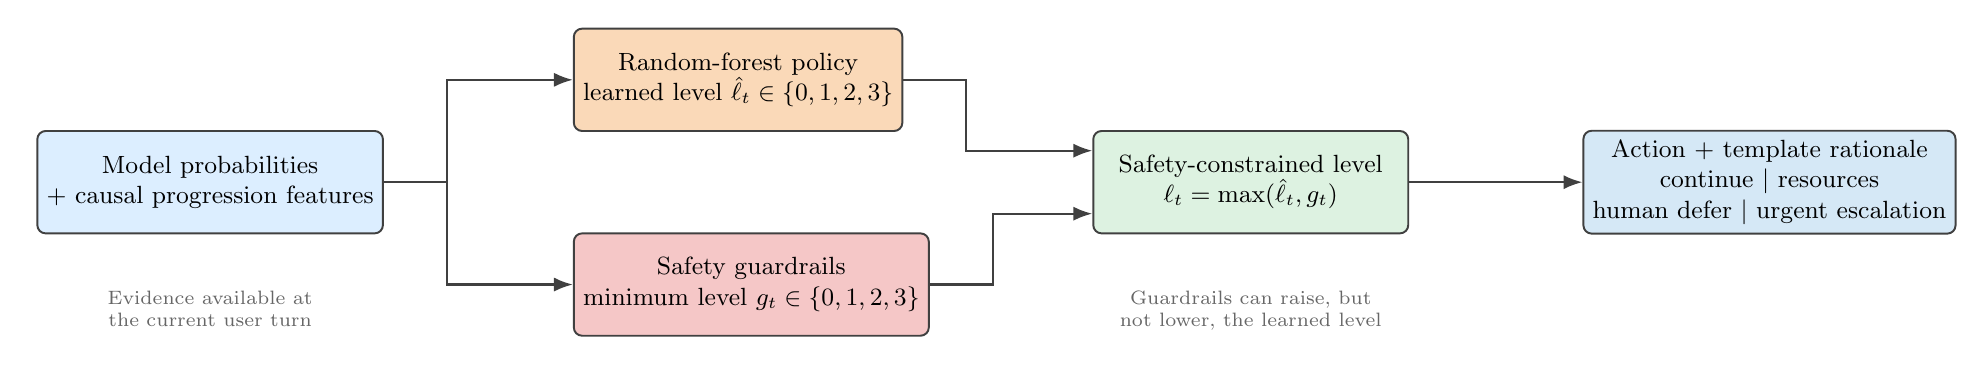
\begin{tikzpicture}[node distance=12mm and 18mm]

\node[block, fill=inputblue, minimum width=42mm] (evidence)
  {Model probabilities\\+ causal progression features};

\node[block, fill=policyorange, right=24mm of evidence, yshift=13mm] (learned)
  {Random-forest policy\\learned level $\hat\ell_t\in\{0,1,2,3\}$};

\node[block, fill=safetyred, right=24mm of evidence, yshift=-13mm] (guard)
  {Safety guardrails\\minimum level $g_t\in\{0,1,2,3\}$};

\node[block, fill=mergegreen, right=24mm of learned, yshift=-13mm,
  minimum width=40mm] (merge)
  {Safety-constrained level\\$\ell_t=\max(\hat\ell_t,g_t)$};

\node[block, fill=outputblue, right=22mm of merge, minimum width=43mm] (output)
  {Action + template rationale\\continue $\mid$ resources\\human defer $\mid$ urgent escalation};

\draw[flow] (evidence.east) -- ++(8mm,0) |- (learned.west);
\draw[flow] (evidence.east) -- ++(8mm,0) |- (guard.west);
\draw[flow] (learned.east) -- ++(8mm,0) |- ([yshift=4mm]merge.west);
\draw[flow] (guard.east) -- ++(8mm,0) |- ([yshift=-4mm]merge.west);
\draw[flow] (merge) -- (output);

\node[note, below=6mm of evidence, text width=44mm]
  {Evidence available at the current user turn};
\node[note, below=6mm of merge, text width=46mm]
  {Guardrails can raise, but not lower, the learned level};

\end{tikzpicture}
\end{document}

